\documentclass[12pt, titlepage]{article}

\usepackage{booktabs}
\usepackage{tabularx}
\usepackage{graphicx}
\usepackage{float}
\usepackage[dvipsnames]{xcolor}

\title{SE 3XA3: Development Plan: Rev 1 \\\textbf{Plagiarism Check}}

\author{Team 310, MXQ Squad
		\\ Mrinal Kumar Tiwari -- tiwarim
		\\ Qifeng Xu -- xuq14
		\\ Xu Wang --  wangx147

}

\date{}



\begin{document}


\maketitle

\newpage

\begin{table}[H]
\caption{Revision History} \label{TblRevisionHistory}
\begin{tabularx}{\textwidth}{11X}
\toprule
\textbf{Date} & \textbf{Developer(s)} & \textbf{Change}\\
\midrule
Jan 23, 2020 & Mrinal, Qifeng, Xu & Added the problem statement: \textcolor{red}{Rev 0} \\
Jan 30, 2020 & Mrinal, Qifeng, Xu & Added the development plan: \textcolor{red}{Rev 0} \\
\textcolor{red}{April 6, 2020}& \textcolor{red}{Mrinal}  & \textcolor{red}{Updated the Problem Statement: Rev 1} \\
\textcolor{red}{April 6, 2020}& \textcolor{red}{Mrinal, Qifeng Xu, Xu Wang}  & \textcolor{red}{Updated the Development  Plan: Rev 1} \\
\bottomrule
\end{tabularx}
\end{table}


\newpage


\section{Team Meeting Plan} 
\textcolor{red}{MXQ Software Development team} would be meeting during regular 3XA3 lab times to work on weekly deliverable. We would also be meeting in person every Thursday evening from 8:00 pm to 9:00 pm to work on the coding part of the project, including implementing new feature, debugging code, adding tests and planning next sprint for the project. \\

\textcolor{red}{The team} would also be doing Discord video meeting to work together on Documentation deliverable. The time for video calls would be decided in the same week as the call through group chat on Facebook messenger. The time decided would best suit schedule of all the team members. \\

\textcolor{red}{The agenda of the meeting would be decided well before meeting and would include documentation, programming or testing dpending on the requirement of the project at the time of the meeting. Mrinal would be acting as team lead, Qifeng would be taking down meeting minutes and all three together would be reviewing each other's work at the end of the meeting.}


\section{Team Communication Plan} 
\textcolor{red}{MXQ Software Development team} would be using a number of methods to communicate depending on the type of communications we need. \textcolor{red}{The team} would be using Facebook Messenger for normal day to day texts and updates while using Discord for working on documentation part of the project. \textcolor{red}{The team} would also be meeting in person during scheduled 3XA3 labs and Thursday night.

\section{Team Member Roles} 
\textcolor{red}{MXQ Software Development team} would be implementing this project on focussing on strengths and weakness of the team members. Mrinal has some prior knowledge of REST, Flask and Docker so he would be using his knowledge to make existing project to ease the hosting of API on the interactive website.  \\*
Qifeng has prior knowledge of HTML CSS and would be helping with the website implementation part.

\begin{table}[]
\caption{Team members role} \label{Team}
\begin{tabularx}{\textwidth}{20X}
\toprule
\textbf{Member} & \textbf{Role} \\
\midrule
Mrinal & \textcolor{red}{Add}  Flask end points\\
\textcolor{red}{Mrinal} & \textcolor{red}{Make} an interactive website \\
\textcolor{red}{Mrinal} & \textcolor{red}{Link} website to the API \\
all & \textcolor{red}{Documentation} \\
\textcolor{red}{Qifeng Xu, Xu Wang} & \textcolor{red}{System Testing} \\
\textcolor{red}{Xu Wang} & \textcolor{red}{Unit Testing} \\
all & \textcolor{red}{Debug} \\
\bottomrule
\end{tabularx}
\end{table}


\section{Git Workflow Plan}
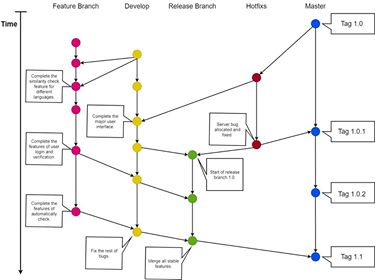
\includegraphics[height=13cm,width=15cm]{workflow.jpg}

\section{Proof of Concept Demonstration Plan} 
Some of the challenges that could be faced by the group are : There might be some difficulties with implementation part. Also, it could be challenging to satisfy all test environment, testing a particular software in a controlled environment is tough. \textcolor{red}{The team is supposed to use system testing, unit testing and survey testing for the whole testing process. Also, for implementation part, decompose the whole project into multiple modules and then implement each module would be a good idea.} \\*


\section{Technology}
\textcolor{red}{MXQ Software Development team} would be mainly using Python3, HTML5, CSS5 and \textcolor{red}{JavaScript} in Visual \textcolor{red}{Studio} Code IDE \textcolor{red}{and Google Chrome web browser} to implement this project. It would also be using a number of testing techniques and frameworks \textcolor{red}{like PyTest, Mocha JavaScript framework} to test the code and debug it. For document generation, \textcolor{red}{the team} would be using Latex and Doxygen. 

\section{Coding Style}
Our code must be as clean and easy to read as possible. Also, our code should have enough comments to make it easy to understand. \textcolor{red}{The team would use curly brace, semicolons, empty line between logical blocks, spaces around operators, a space between parameters in coding. And the lines should not be too long.}

\section{Project Schedule}

https://gitlab.cas.mcmaster.ca/wangx147/3xa3-project/blob/master/Project\_Schedule/3XA3\_Project\_schedule.gan

\section{Project Review}

\end{document}
